\chapter{Funções de Perda para Usos Específicos}
\label{cap:perdas-especificas}

\section{Focal Loss} \index{Funções de Perda!Focal Loss}

\begin{equacaodestaque}{Focal Loss}
    \Loss_{\text{FL}}(p_t) = -(1 - p_t)^\gamma \log(p_t)
    \label{eq:focal-loss}
\end{equacaodestaque}

\begin{figure}[h!]
    \centering
    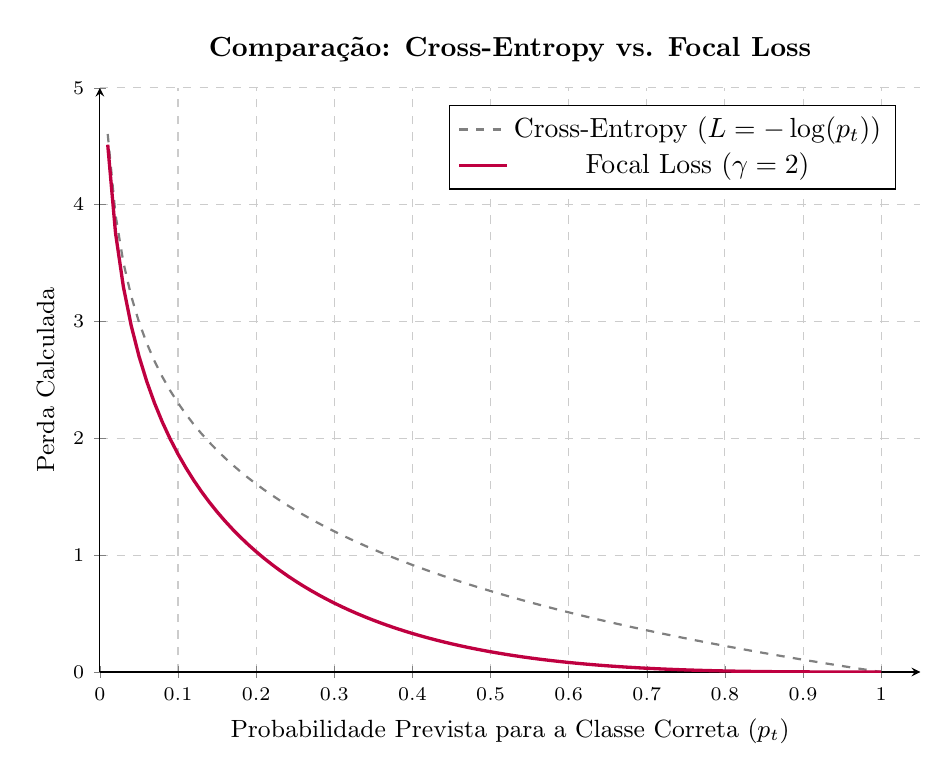
\begin{tikzpicture}
        \begin{axis}[
            title={Comparação: Cross-Entropy vs. Focal Loss},
            xlabel={Probabilidade Prevista para a Classe Correta ($p_t$)},
            ylabel={Perda Calculada},
            axis lines=left,
            grid=major,
            grid style={dashed, gray!40},
            xmin=0, xmax=1.05,
            ymin=0, ymax=5,
            legend pos=north east,
            width=12cm,
            height=9cm,
            title style={font=\bfseries},
            label style={font=\small},
            tick label style={font=\scriptsize}
        ]
            % Cross-Entropy Padrão
            \addplot[
                domain=0.01:1, samples=100, color=gray, dashed, thick
            ] {-ln(x)};
            \addlegendentry{Cross-Entropy ($L = -\log(p_t)$)}

            % Focal Loss com gamma=2
            \addplot[
                domain=0.01:1, samples=100, color=purple, very thick
            ] {-(1-x)^2 * ln(x)};
            \addlegendentry{Focal Loss ($\gamma=2$)}
            
        \end{axis}
    \end{tikzpicture}
    \caption{Gráfico da Focal Loss em comparação com a Entropia Cruzada padrão. A perda para exemplos fáceis ($p_t \to 1$) é drasticamente reduzida.}
    \label{fig:focal-loss}
    \fonte{O autor (2025).}
\end{figure}

\begin{equacaodestaque}{Derivada da Focal Loss}
    \frac{\partial \Loss_{\text{FL}}}{\partial z} = 
    \begin{cases} 
        \hat{y}(\gamma(1-\hat{y})\log(\hat{y}) + \hat{y} - 1) & \text{se } y=1 \\
        (1-\hat{y})(\gamma\hat{y}\log(1-\hat{y}) + \hat{y}) & \text{se } y=0
    \end{cases}
    \label{eq:focal-loss-derivada}
\end{equacaodestaque}

\begin{figure}[h!]
    \centering
    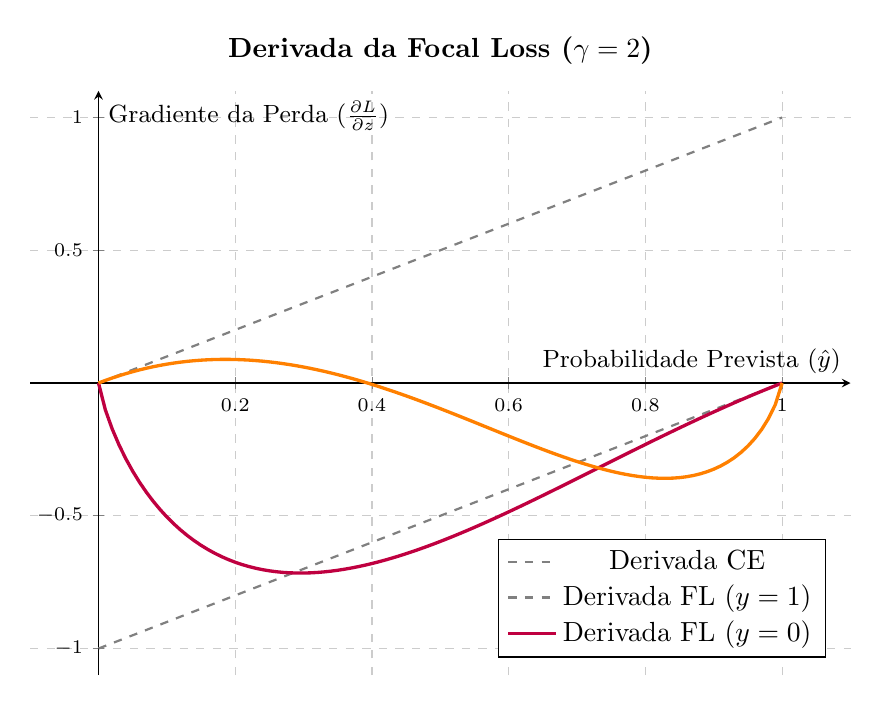
\begin{tikzpicture}
        \begin{axis}[
            title={Derivada da Focal Loss ($\gamma=2$)},
            xlabel={Probabilidade Prevista ($\hat{y}$)},
            ylabel={Gradiente da Perda ($\frac{\partial L}{\partial z}$)},
            axis lines=middle,
            grid=major,
            grid style={dashed, gray!40},
            xmin=-0.1, xmax=1.1,
            ymin=-1.1, ymax=1.1,
            legend pos=south east,
            width=12cm,
            height=9cm,
            title style={font=\bfseries},
            label style={font=\small},
            tick label style={font=\scriptsize}
        ]
            % Derivada da Cross-Entropy padrão (y_hat - y)
            \addplot[domain=0:1, samples=10, color=gray, dashed, thick] {x-1};
            \addplot[domain=0:1, samples=10, color=gray, dashed, thick] {x};
            \addlegendentry{Derivada CE}
            
            % Derivada da Focal Loss para y=1
            \addplot[
                domain=0:1, samples=101, color=purple, very thick
            ] {x*(2*(1-x)*ln(x) + x - 1)};
            \addlegendentry{Derivada FL ($y=1$)}

            % Derivada da Focal Loss para y=0
            \addplot[
                domain=0:1, samples=101, color=orange, very thick
            ] {(1-x)*(2*x*ln(1-x) + x)};
            \addlegendentry{Derivada FL ($y=0$)}
            
        \end{axis}
    \end{tikzpicture}
    \caption{Gráfico da derivada da Focal Loss. O gradiente para exemplos fáceis (próximo das bordas 0 e 1) é suprimido em comparação com a derivada da Entropia Cruzada padrão.}
    \label{fig:focal-loss-derivada}
    \fonte{O autor (2025).}
\end{figure}

\medskip
\begin{center}
 * * *
\end{center}
\medskip

\textbf{Algumas Aplicações da \textit{Focal Loss}}
\vspace{1em}

\begin{itemize}
    \item \textbf{Aplicação 1 (Área):}
    \item \textbf{Aplicação 2 (Área):}
    \item \textbf{Aplicação 3 (Área):}
    \item \textbf{Aplicação 4 (Área):}
\end{itemize}

\medskip
\begin{center}
 * * *
\end{center}
\medskip

\section{Fluxograma:}
